\documentclass{article}

% Language setting
% Replace `english' with e.g. `spanish' to change the document language
\usepackage{biblatex} %Imports biblatex package
\addbibresource{sample.bib}
\usepackage[english]{babel}
\usepackage{array}
\usepackage{amsmath}
\usepackage{pythonhighlight}
\newcolumntype{P}[1]{>{\centering\arraybackslash}p{#1}}
\newcolumntype{M}[1]{>{\centering\arraybackslash}m{#1}}

% Set page size and margins
% Replace `letterpaper' with `a4paper' for UK/EU standard size
\usepackage[letterpaper,top=2cm,bottom=2cm,left=3cm,right=3cm,marginparwidth=1.75cm]{geometry}

\usepackage{amsmath}
\usepackage{graphicx}
\usepackage[colorlinks=true, allcolors=blue]{hyperref}
\usepackage{setspace}
\usepackage{booktabs}
\usepackage[T1]{fontenc}
\usepackage{longtable}
\doublespacing

\begin{document}
\begin{titlepage}

\centering
\scshape
\vspace{\baselineskip}

%
\rule{\textwidth}{1.6pt}\vspace*{-\baselineskip}\vspace*{2pt}
\rule{\textwidth}{0.4pt}

{\Huge \textbf{\textsc{NPRE 449: Homework 3 \\
\vspace{15pt}}}}

\rule{\textwidth}{0.4pt}\vspace*{-\baselineskip}\vspace{3.2pt}
\rule{\textwidth}{1.6pt}\vspace{6pt}
%%\centerline{\textit{University of Illinois at Urbana-Champaign}} 
\vspace{1.5\baselineskip}


\large \centerline{\textbf{Author:} Nathan Glaser}
\large \centerline{\textbf{Net-ID:} nglaser3}
\quad

\vfill
\large \centerline{September 18, 2024}
%
\pagenumbering{gobble}
\end{titlepage}

\tableofcontents
\newpage
\pagenumbering{arabic}

\section*{Question 1}
\addcontentsline{toc}{section}{\protect\numberline{}Question 1}

A Pressurized Water Reactor (PWR) is a variant of a Light Water Reactor (LWR). This reactor type utilizes light water (Standard $H_2O$ as opposed to $D_2O$) as both its coolant and moderator. This water is highly pressurized, typically at 15.5 MPa. This pressurization is to increase the boiling point of saturated water, reducing the amount of boiling occurring inside the reactor core itself, ensuring water is constantly in contact with the hot surfaces in the core. the reactor vessel will have between 2 and 4 pairs of pipes (for systems using U-Tube steam generators, Once-Through steam generators have 1 hot leg for two cold legs), termed hot and cold legs. Each inlet cold leg will have an outlet hot leg; both are at the same elevation with respect to the reactor core. Water enters the reactor vessel through the cold legs and through the down-comer, which forces the water into the lower-plenum below the reactor core. From here, the water is forced up through the reactor core, and out through the hot legs. Notably, the control rods of PWRs are above the reactor when not in use. The fuel of PWRs is of the form of $UO_2$ cylindrical pellets, formed into long rods. Each rod is typically clad with some rendition of Zircalloy. These rods are then placed into square assemblies with somewhere around 17x17 rods, depending on the design of the core. Each assembly is actually an 'open' structure, meaning cross-flow between assemblies is able to occur. The flow path of a PWR is presented in Fig. \ref{fig:pwr}:

\begin{figure}[!h!]
    \centering
    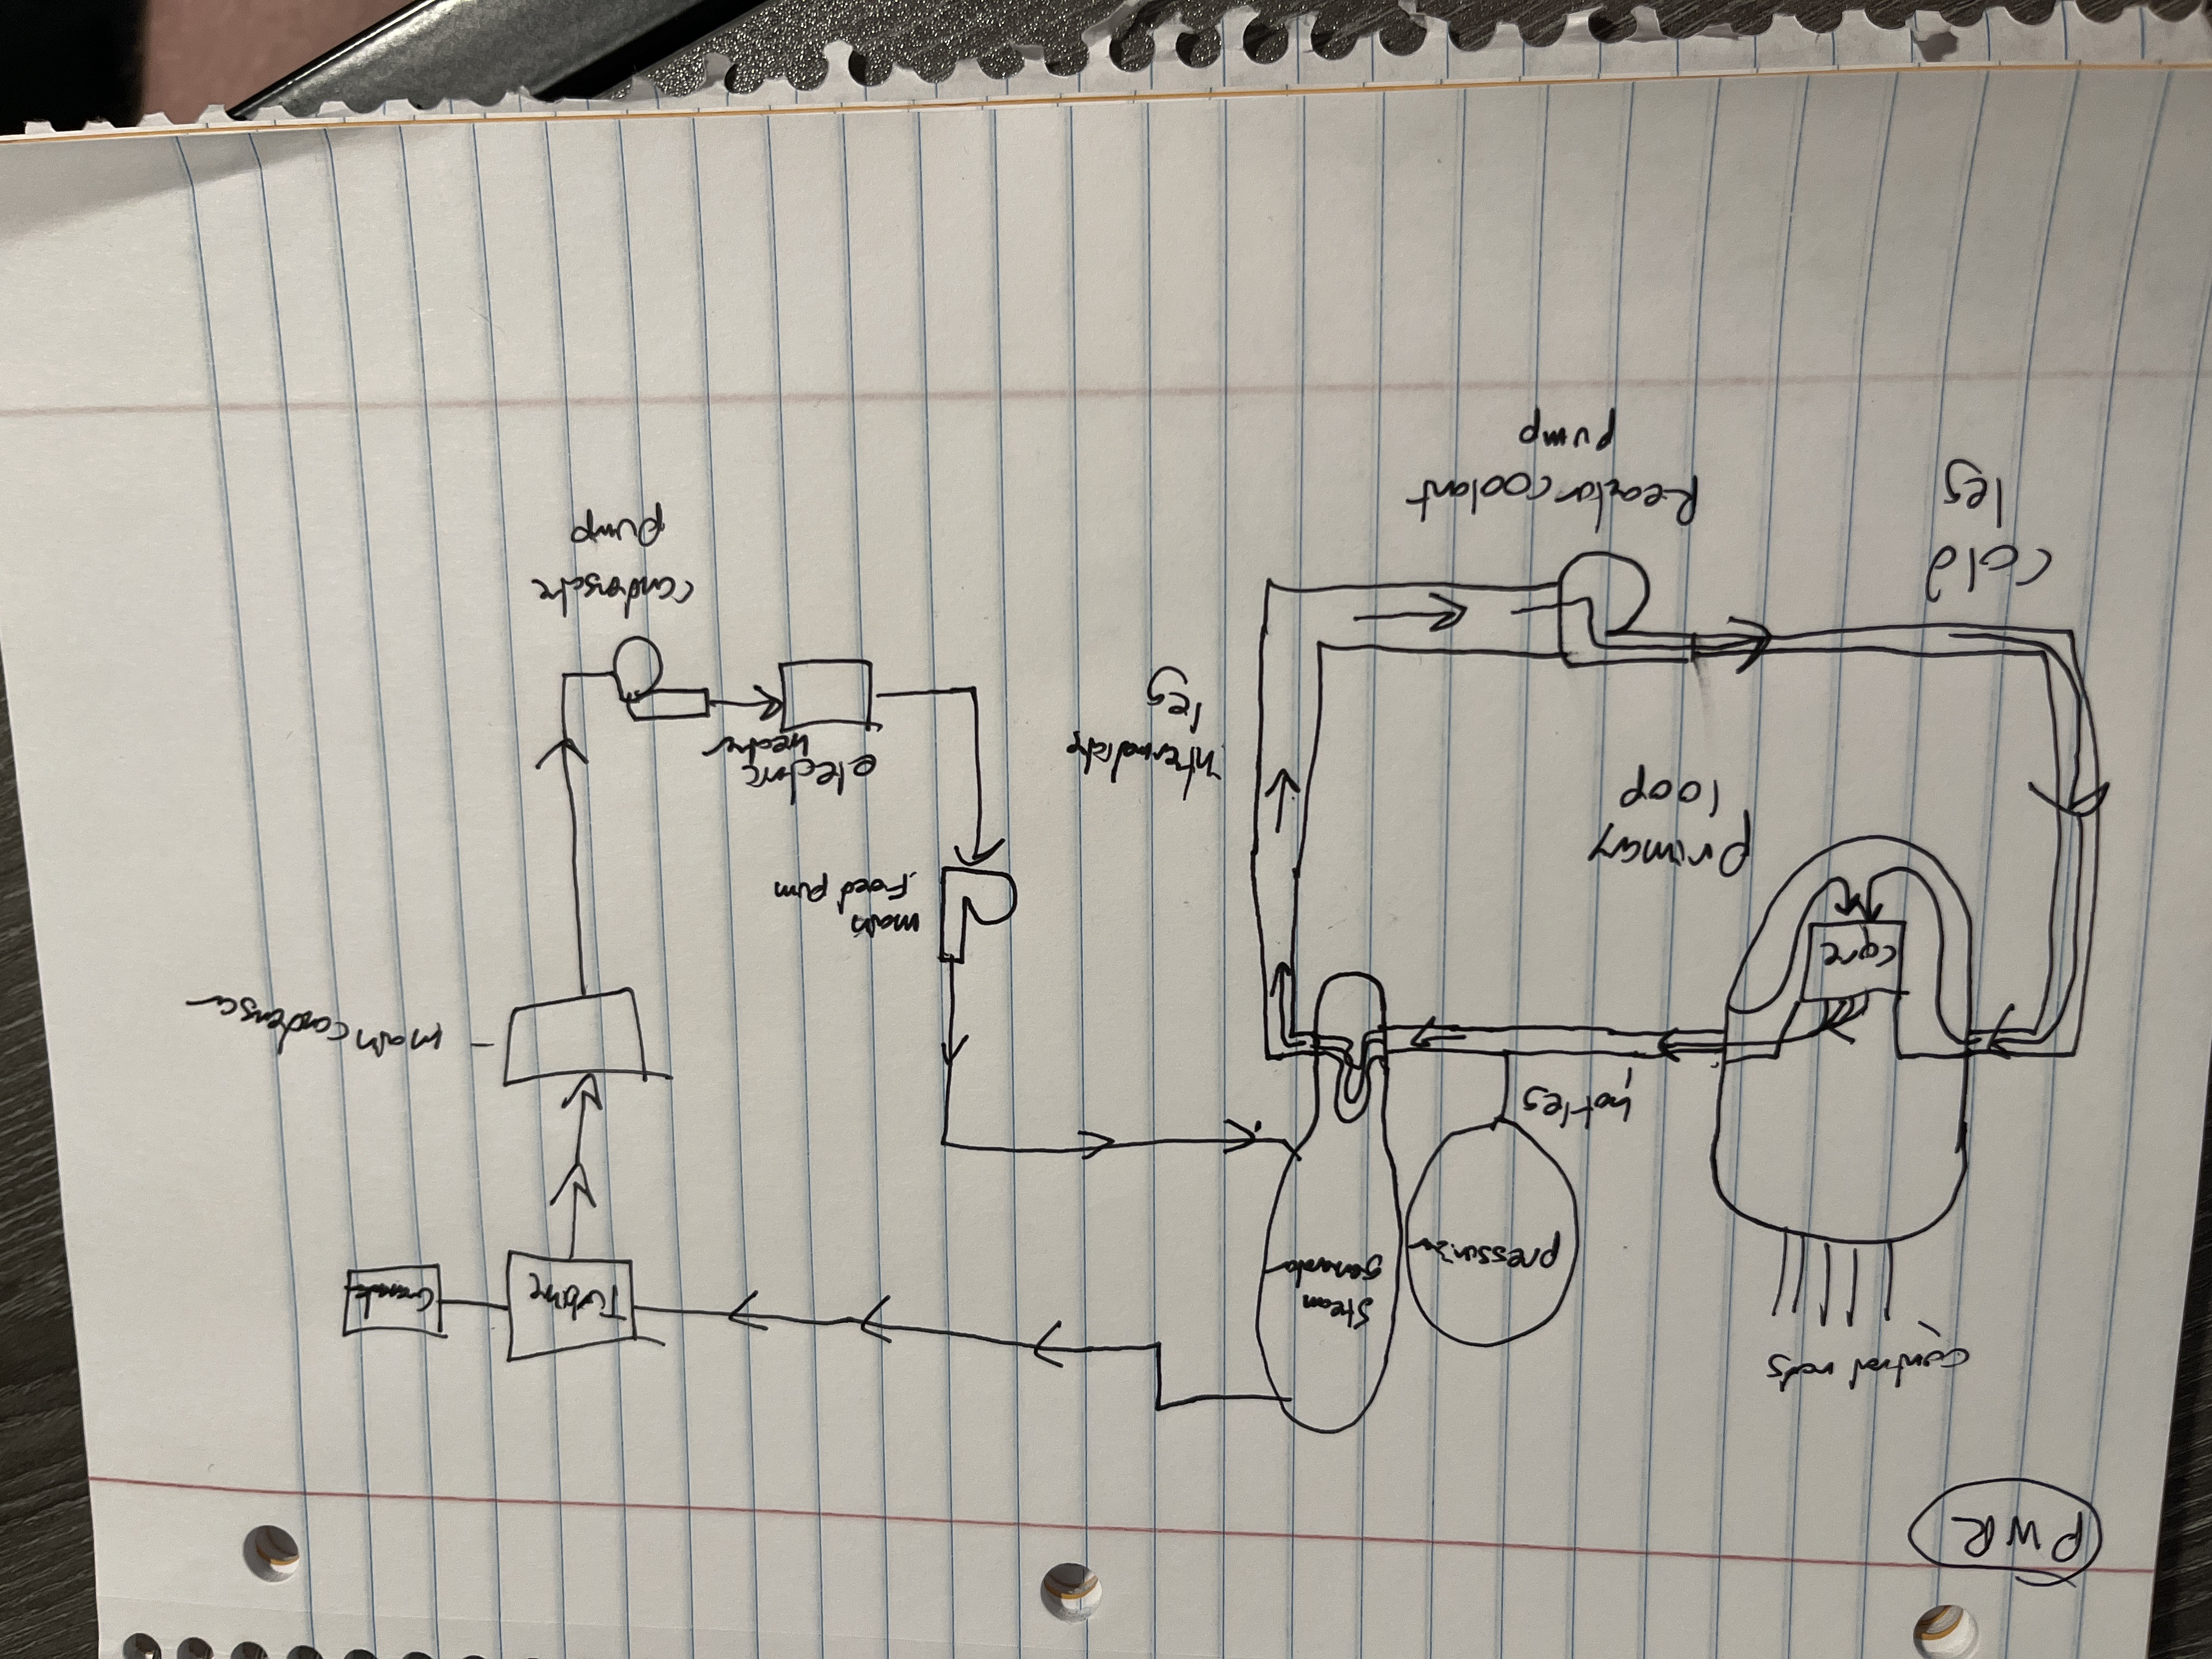
\includegraphics[width=0.9\linewidth,angle=180]{hw3PWR.JPG}
    \caption{Flow path of prototypical PWR}
    \label{fig:pwr}
\end{figure}

\newpage
Within the primary loop there are four main components, excluding the piping. There is the reactor vessel, the pressurizer, the steam generator, and the reactor coolant pump. The hot legs connects the reactor vessel to the pressurizer to the steam generator; the intermediate leg connects the steam generator to the reactor coolant pump; and the cold leg connects the reactor coolant pump to the reactor vessel. The reactor vessel heats the incoming water to near-saturation temperatures. The pressurizer simply maintains the pressure in the piping, allowing operator control. The steam generator, depending on the model, takes in the hot water from the reactor and transfers the heat to the secondary loop, creating steam. There are two standard steam generators: U-Tube and Once-Through. U-Tube steam generators involve segregating inlet hot reactor water into thousands of small tubes, and then running cold secondary loop water over these tubes; then running the heated secondary loop water through driers and separators. The maximum steam quality achieved is .9975. Once-Through steam generators are much more complex internally, having one hot leg outlet and two cold leg inlets. This steam generator type is essentially a heat exchanger, and can super heat vapor, thus achieving steam qualities greater than 1. Finally, the reactor coolant pump has a volumetric flow rate of roughly 100,000 gallons per minute, utilizing a motor with 6-10,000 horsepower. 


\newpage
\section*{Question 2}
\addcontentsline{toc}{section}{\protect\numberline{}Question 2}

A Boiling Water Reactor (BWR) is another variant of a LWR. BWRs utilize the same coolant / moderator as PWRs. The pressure in BWRs is roughly half of PWRs --- in BWRs we want the water to boil in the core. BWRs differ from PWRs mainly in that the steam generator is actually combined with the core. There is no distinct primary and secondary loop, at least as far as for energy production. To begin, water comes in through the feed water lines and down over the jet-pumps. The jet pumps are designed to have high fluid velocity, pulling water down through them. This occurs due to low pressures normal to the flow direction of the fluid. However, not all incoming fluid from the feed water pumps go through the jet pumps initially. The water that does not go through the jet pumps is recirculated out of the reactor vessel through the recirc pump lines and down through jet pumps again. From here, the water flows up through the core and boils. After exiting the core, the steam quality is roughly 0.15-0.20, and here it enters the steam dome. The water is then pushed through driers and seperators, achieving an exit steam quality of 0.997. This resulting steam is then sent out of the reactor vessel through the main stea line, sent out of containment, and through the turbine. Much like in a PWR, after leaving the Turbine the steam passes through the main condensor, then through a feedwater pump, and then through an electric heater. After the water is sent through the electric heater it is then sent back through the core. The fuel form of BWRs is similair to PWRs --- $UO_2$ fuel pellets stacked into rods. The assembly structure of BWRs is rather different however, and so is the control 'rods'. BWR fuel assemblies have fewer rods per assembly, typically 8x8 rods, and are 'canned' (laterally sealed) so as to not allow lateral flow through the core. Lateral flow is bad in BWRs because bubbles tend to 'drift' towards the center of the core, which would cause poor heat transfer at the most fission-productive region of the core. Further, the control 'rods' in BWRs are actually blades, and are inserted in the open space between the fuel assemblies and are of the shape of '+'. Also, these control blades are, when withdrawn, below the core and are thus susceptible to insertion failure (PWRs rely on gravity, with magnets holding the control rods up). Because of this potential failure source, BWRs have a back-up system for control rods --- the standby liquid control system. Further, unlike PWRs BWRs have pumps in their high pressure ECCS that do not require external power as they are driven by their own turbines. Consequentially, BWRs when undergoing a station blackout event do not want to vent and de-pressurize the reactor vessel. Typical BWR flow path is presented in Fig. \ref{fig:bwr}:

\begin{figure}[!h!]
    \centering
    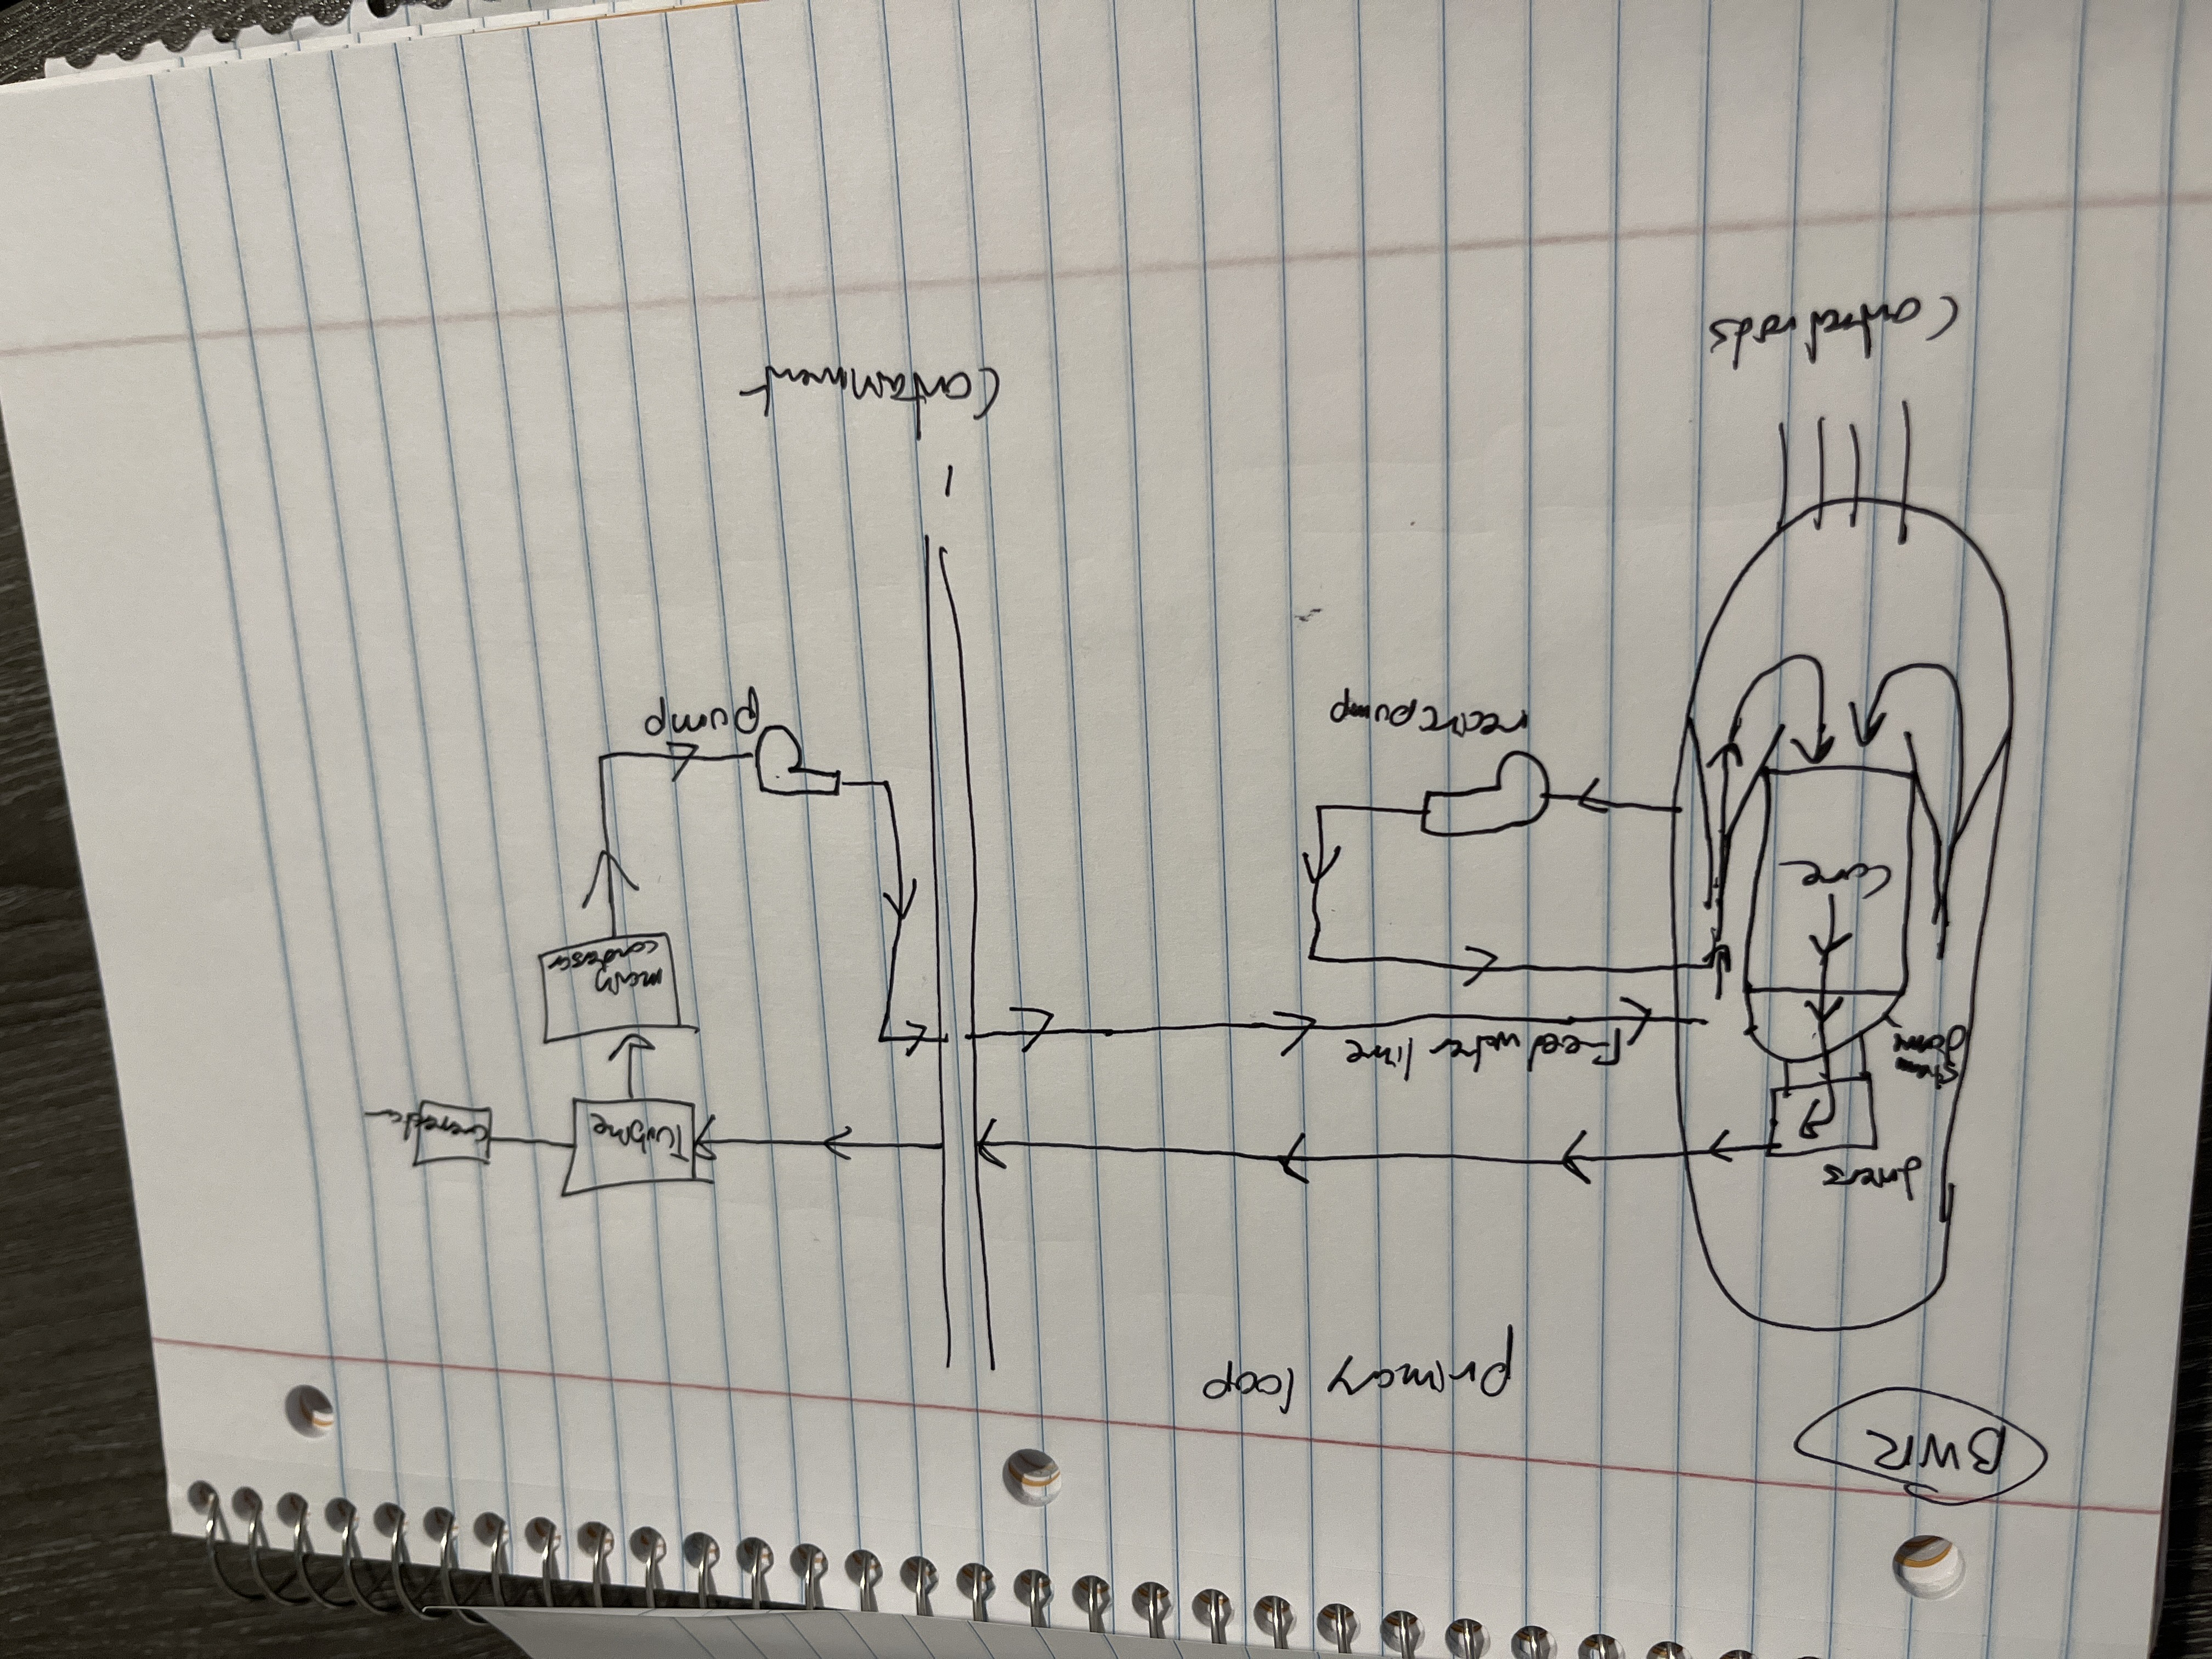
\includegraphics[width=0.9\linewidth,angle=180]{hw3BWR.JPG}
    \caption{Flow path of prototypical BWR}
    \label{fig:bwr}
\end{figure}

\newpage
The primary loop of a BWR technically includes the secondary-loop components of PWRs, but is typically defined as the portion of the main loop within containment. Thus, the primary loop of a BWR contains the feed-water line, the core, the steam dome, the driers \& separators, and the main steam line. The feed-water line contains near-saturated water (heated by the electric heaters outside of containment). The reactor core boils the incoming water and sends it to the steam dome, where the steam is shoved through driers and separators before exiting through the main steam line. 


\newpage
\section*{Question 3}
\addcontentsline{toc}{section}{\protect\numberline{}Question 3}

Thermal design limits, pertaining to PWRs and BWRs, are operational limitations on the reactors themselves due to material limitations. In nuclear systems, these thermal design limits are the limiting factor for power output, not fuel energy density. For both PWR and BWR systems, the main thermal design limitation is due to boiling water.  In both systems, other than the water, the fuel and Zircaloy cladding have thermal limits as well. For Zircaloy the cladding cannot reach 1204 $^o$C, as at this temperature the cladding oxidizes, which is a very exothermic reaction releasing 190 kJ/mol. Further, the fuel itself has a melting temperature of 2865 $^o$C, and cannot operate higher than this temperature due to changes in fissile density.  

For PWRs, the thermal design limit attributed to boiling water is called Departure from Nucleate Boiling (DNB). This occurs when water cannot physically reach the surface. This is very low-quality steam, essentially inverse of annular flow in BWRs. There is a thin steam layer directly on the surface, and immediately outside of this layer is liquid water.

For BWRs, the thermal design limit from water is called Dryout. Dryout is the point in which there is no longer any water contact with the wall. At this point the coolant is high-quality steam, that is to say that the steam contact with the surface is not simply a boundary but the entirety of the coolant. 

A thermal design margin is the ratio of the minimum parameter that causes the thermal design limit to the maximum of that parameter in your reactor system. Essentially, if you have a thermal design margin of 1.3, then the heat-flux required to reach the limit is 1.3 times, or 30\%, greater than the maximum heat-flux in your system. This is done to ensure that the thermal limitations of your system are not reached when under standard operations. Typical values for DNB are 1.3, and typical values for Dryout are 1.2-1.3. 

\newpage
\section*{Question 4}
\addcontentsline{toc}{section}{\protect\numberline{}Question 4}

To begin, the relevant equations are presented below in Eq. \ref{eq:2.5}:
\begin{equation}
    \Dot(Q) = NL \left< q' \right> = NL\pi D_{co} \left< q''_{co}\right> = NL\pi R_{fo}^2 \left< q''' \right>
    \label{eq:2.5}
\end{equation}

And then from this equation we can find relations between $q'$, $q''_{co}$, and $q''$:
\begin{equation}
    q' = \pi D_{co} \left< q''_{co} \right> = \pi R_{fo}^2 \left< q''' \right>
    \label{eq:q4}
\end{equation}

All Volumetric heat rates ($q'''$) and heat fluxes ($q''$) are tabulated below:
\vspace{20pt}

\begin{tabular}{|c|c|c|c|c|c|c|}
    \toprule
     & BWR & PWR & PHWR & HTGR & AGR & LMFBR \\
     \midrule
     Linear Heat Rate ($q'$) [kw] & 19.0 & 17.8 & 25.7 & 7.87 & 17.0 & 29.0\\
     Clad Diameter $D_{co}$ [mm] & 12.27 & 9.5 & 13.1 & 15.7 & 14.89 & 8.65\\
     Fuel Radius $R_{fo}$ [mm] & 5.2 & 4.1 & 6.1 & 7.85 & 7.255 & 3.5 \\ 
     \midrule
     $q'''$, Eq. \ref{eq:q4} $\left[\frac{MW}{m^3}\right]$ & 223.6644 & 337.0562 & 219.8485 &  40.6523 & 102.8073 & 753.5499 \\
     $q''$, Eq. \ref{eq:q4} $\left[\frac{kW}{m^2}\right]$ & 492.9003 &  596.4122 & 624.4705 & 159.5604 & 363.4162 & 1067.1660 \\ 
     \bottomrule
         
\end{tabular}

\vspace{20pt}
\section*{Question 5}
\addcontentsline{toc}{section}{\protect\numberline{}Question 5}

To begin, the margin is defined by:
\begin{equation}
    margin = \frac{failure limit}{maximum expected}
\end{equation}

Further, the maximum expected is simply the average linear heat power multiplied by the multiplication factors: Radial Flux (1.55), Axial and Local Flux Factor (1.70), Engineering Uncertainty Factor (1.05), and Overpower Factor (1.15).

\begin{equation}
    limit = 17.8 \cdot 1.55 \cdot 1.70 \cdot 1.05 \cdot 1.15 = 56.6353725
\end{equation}

and then: 

\begin{equation}
    \frac{70.0}{56.6353725} = 1.2359766
\end{equation}

\end{document}
